\documentclass{article}
\usepackage[utf8]{inputenc}
\usepackage{amsthm}
\usepackage{amsmath, mathtools, amsfonts,amssymb}
\usepackage{graphicx}
\usepackage{verbatim}
\usepackage{fancyhdr}
% Code
\usepackage{listings} 
\usepackage{algorithm}
\usepackage{algpseudocode}
\usepackage{color}
% Margins
\usepackage{geometry}
%\usepackage{enumitem} % for nice enumerating
\geometry{margin=1in}

% Graphics
\usepackage{tikz}
\usetikzlibrary{matrix} % matrices
\usepackage{tikz-qtree} % Simple trees
\usepackage{verbatim} % what is this for again???

\setcounter{section}{-1}

\newtheorem{pic}{Figure}
\numberwithin{pic}{section}
\newtheorem{lem}{Lemma}
\numberwithin{lem}{section}
\newtheorem{thm}{Theorem}
\numberwithin{thm}{section}
\newtheorem{cor}{Corollary}
\numberwithin{cor}{section}

\theoremstyle{definition}
\newtheorem{ex}{Example}
\numberwithin{ex}{section}
\newtheorem{defn}{Definition}
\numberwithin{defn}{section}
\theoremstyle{definition}
\newtheorem{prob}{Problem}

\theoremstyle{remark}
\newtheorem*{con}{Conjecture}
\newtheorem{rem}{Remark}
\newtheorem*{cex}{Counterexample}
\newtheorem*{ts}{T.S.}

\lstset{frame=tb,
  language=c,
  aboveskip=3mm,
  belowskip=3mm,
  showstringspaces=false,
  columns=flexible,
  basicstyle={\small\ttfamily},
  numbers=none,
  numberstyle=\tiny\color{gray},
  keywordstyle=\color{blue},
  commentstyle=\color{violet},
  stringstyle=\color{brown},
  breaklines=true,
  breakatwhitespace=true,
  tabsize=3
}

%%% COMMANDS %%%
% Sets
\newcommand{\set}[1]{\ensuremath{\left\{ #1\right\}}} % write sets
\newcommand{\e}{\ensuremath{\epsilon}} % Epsilon
\newcommand{\R}{\ensuremath{\mathbb{R}}} % Real Numbers
\newcommand{\N}{\ensuremath{\mathbb{N}}} % Natural numbers
\newcommand{\Q}{\ensuremath{\mathbb{Q}}} % Rationals
\newcommand{\I}{\ensuremath{\mathbb{I}}} % Irrational Numbers
\newcommand{\Z}{\ensuremath{\mathbb{Z}}} % Integers
% Easier Delimiters?
\newcommand{\lr}[2]{\ensuremath{\left#1 #2 \right #1}}
% Absolute Value
\newcommand{\abs}[1]{\ensuremath{\left| #1 \right|}}
% Landau Notation
\newcommand{\Oh}{\ensuremath{\mathcal{O}}} %%% IN MATH MODE
\newcommand{\oh}{\ensuremath{\mathcal{o}}} %%% IN MATH MODE
% Display style fractions
\newcommand{\Frac}[2]{\displaystyle \frac{#1}{#2}}
% Display style limits
\newcommand{\Lim}[2]{\displaystyle \lim_{#1}{#2}}

% Enumerate
\renewcommand{\labelenumi}{(\alph{enumi})}
\renewcommand{\labelenumii}{\roman{enumii}}

% change proof environment
\renewcommand*{\proofname}{Pf}

% Indentation
\newlength\tindent
\setlength{\tindent}{\parindent}
\setlength{\parindent}{0pt}
\renewcommand{\indent}{\hspace*{\tindent}}

% Set title
\title{X}

\begin{document}


\fancyhead[l]{Quinn Stratton}
\fancyhead[c]{Nate CS Assignment 1 Alleged Solutions}
%\fancyhead[r]{\today}
\pagestyle{fancy}

\begin{prob}
  
\end{prob}

\begin{prob}
  \lstinputlisting{numberFun.c}
\end{prob}
\begin{prob}
  \lstinputlisting{divisionAlg.c}
\end{prob}
\begin{prob} Here's a truth table argument for the first law.\\
  \begin{center}
  \begin{tabular}{c c | c c | c c c}
    $P$ & $Q$ & $P \vee Q$ & $\neg(P \vee Q)$ & $\neg P$ & $\neg Q$ & $\neg P \wedge \neg Q$\\
    \hline
    F & F & F & \textbf{T} & T & T & \textbf{T}\\
    F & T & T & \textbf{F} & T & F & \textbf{F}\\
    T & F & T & \textbf{F} & F & T & \textbf{F}\\
    T & T & T & \textbf{F} & F & F & \textbf{F}
  \end{tabular}
\end{center}
Since the output of both expressions is the same for all possible assignment of truth values to $P$ and $Q$, $\neg(P \vee Q) \iff \neg P \wedge \neg Q$.
\end{prob}

\begin{prob}
  \begin{align*}
    f(20) &= 20\cdot f(10) &&\text{Since }20 \mod 2 = 0\\
          &= 20\cdot 10\cdot f(5) &&\text{Since }10\mod 2 = 0\\
          &= 20\cdot 10(5 + f(4)) &&\text{Since }5\mod 2 = 1\\
          &= 20\cdot 10(5 + 4\cdot f(2)) &&\text{Since }4\mod 2 = 0\\
          &= 20\cdot 10(5 + 4\cdot 2 \cdot f(1)) &&\text{Since }2\mod 2 = 0\\
          &= 20\cdot 10(5 + 4\cdot 2 \cdot 1) &&\text{Since }1 = 1\\
          &= 20\cdot 10(5 + 8) && \\
          &= 200(13) && \\
          &= 260 &&
  \end{align*}
\end{prob}

\begin{prob}
  \begin{enumerate}
  \item Note that the $foo$ definition seems to deal with the start end end characters of a given string. $aba$ is not the empty string so we will check the other clauses. Since the starting and ending characters of $aba$ are $a$, and $a$, we will proceed with the clause $a\circ foo \circ a$. From here we must examine the substring left after removing the starting and ending characters from $aba$, which is $b$. $b$ does not fit any of the clauses in the $foo$ definition, so $aba$ cannot be a $foo$.
  \item Proceeding as above, $babb$ is clearly not the empty string, but it seems to fit the clause $b\circ foo\circ b$. Looking at the $foo$ definition again, we can further break this down into $b\circ a\circ foo \circ b\circ b$. We can now use the empty string clause leaving us with $b\circ a\circ \epsilon\circ b\circ b = babb$. So $babb$ is a $foo$. This process can be organized using a tree.
    \begin{equation*}
      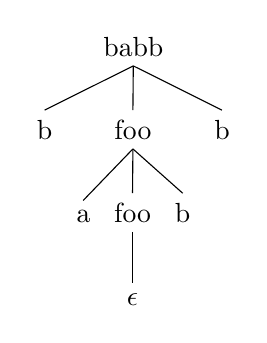
\begin{tikzpicture}
        \Tree [.babb b [.foo a [.foo $\e$ ] b ] b ]
      \end{tikzpicture}
    \end{equation*}
  \item Every case in our $foo$ definition involves either the empty string or a string made of some combination of the characters $a$ and $b$ and another $foo$. The key to describing what a $foo$ is is to realize that anything that is a $foo$ will successfully go through the process outlined in part (b) and so will end up being some number of $a$s and $b$s concatenated together. So we should look at the $a$s and $b$s in the cases of our $foo$ definition and try to notice a pattern. In each case, there are always two literal characters or the empty string, so the length of any $foo$ will be even (we can also see this by examining the process in part (b) which pairs off $a$s and $b$s). The order of the $a$s and $b$s does not really matter since the cases cover every size two permuation of $a$ and $b$ (e.g. $aa$, $ab$, $ba$, $bb$). So a $foo$ is any even length string of $a$s and $b$s.
  \end{enumerate}
  \begin{rem}
    In the field of \textit{Formal Language Theory}, the set of all $foo$s could be considered a \textit{language} with the \textit{alphabet} $\set{a,b}$. I defined a $foo$ in a way that is similar to a \textit{context-free grammar}, which is what the $foo$ language is. Context-free grammars are very useful throughout computer science, mathematics, and linguistics for their ability to mathematically describe the behavior of certain languages.
  \end{rem}
\end{prob}

\end{document}